% !Mode:: "TeX:UTF-8"

\chapter{项目设计}
\section{实现形式}

在最初的设计中,我们预计使用两种方式来实现我们对室内设备的控制,以及显示对室内环境状况的监测。一个是移动端的Android APP,另一个是Web端的网页。预期设计的界面如下:

\begin{figure}[htbp]
\centering
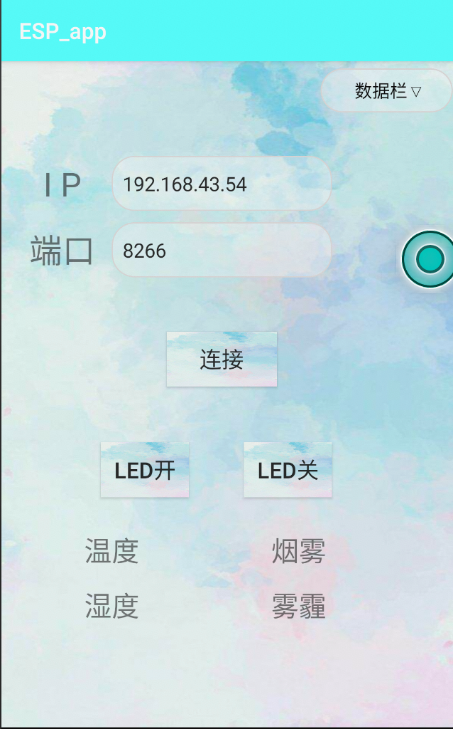
\includegraphics[width=0.3\textwidth]{figures/app_UI}
\caption{App界面}\label{fig:1}
\end{figure}

\begin{figure}[htbp]
\centering
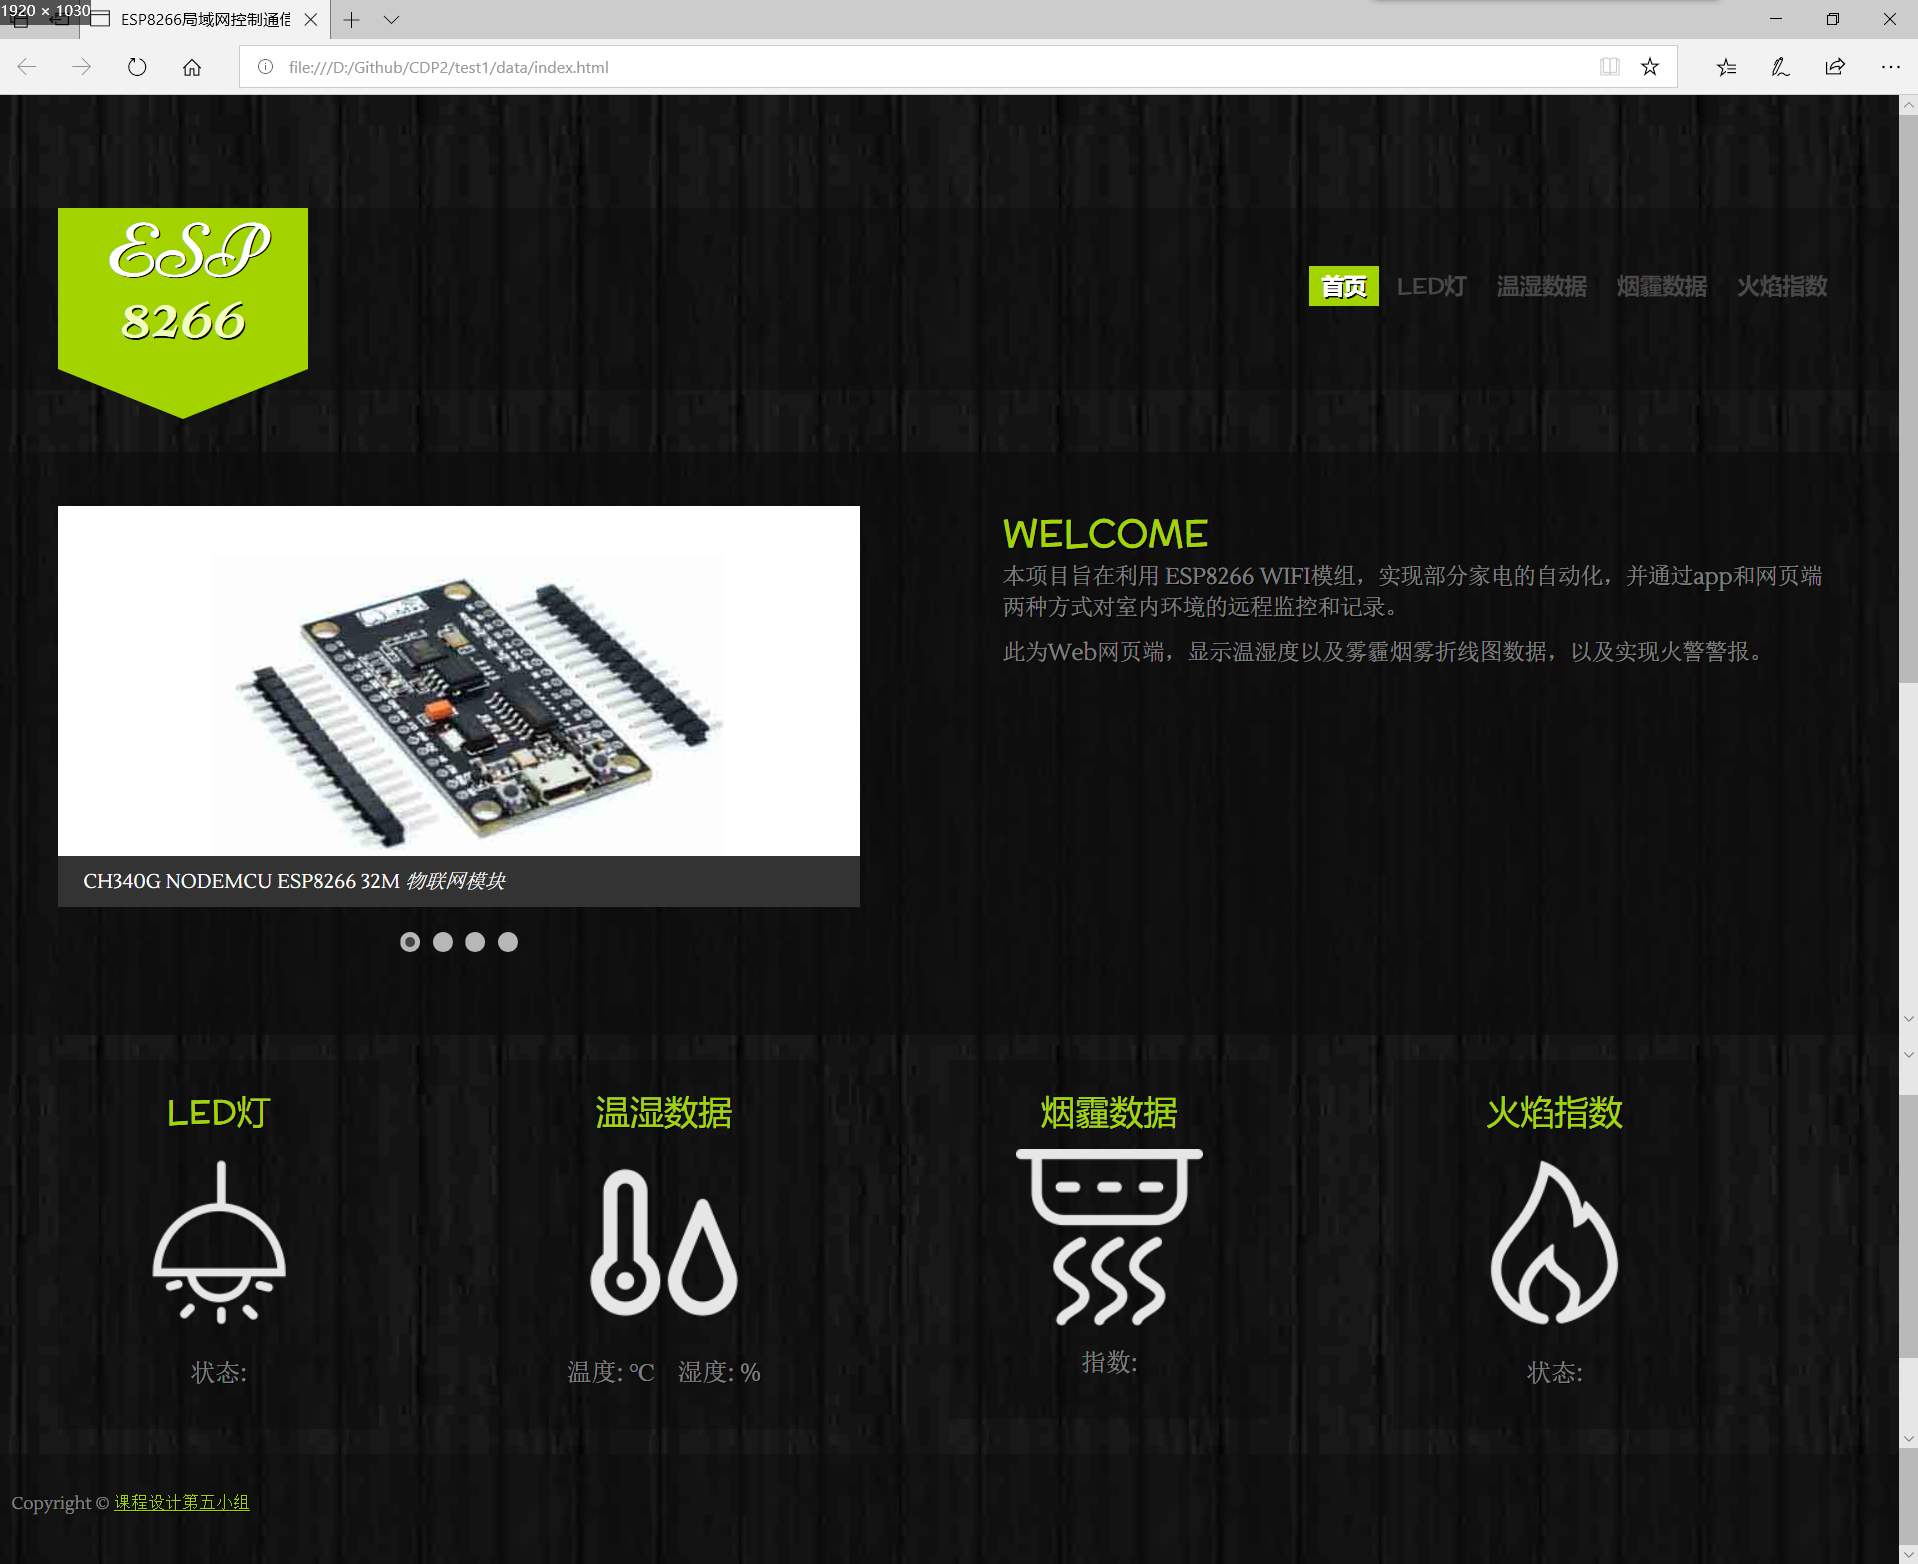
\includegraphics[width=0.7\textwidth]{figures/web_UI}
\caption{Web界面}\label{fig:2}
\end{figure}

\section{使用器材}

\begin{enumerate}
    \item {单片机ESP8266物联网模块}: 
    
    在项目设计的实际相关内容中,核心的部件是单片机ESP8266物联网模块,通过在其中烧录代码,使它能够对移动端app或者是web端发送的指令进行响应,并将传感器读取的数据传回app或是web上。实物如下:
    \begin{figure}[htbp]
    \centering
    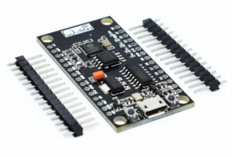
\includegraphics[width=0.3\textwidth]{figures/esp8266}
    \caption{CH340G NODEMCU ESP8266 32M 物联网模块}\label{fig:3}
    \end{figure}

    \item {温湿度传感器}:
    
    对于室内环境状况检测的功能设计中,我们设计了对温度和湿度数据的采集和记录功能。主要采用的是传感器DHT11 温湿度传感器(实物如下图)。通过DHT11 温湿度传感器获取了温度和湿度数据后,再通过ESP8266传回移动端app与web端,使其能够直观地显示出来。除了可以获取当前的温度和湿度数据。我们同样再app和web网页上设计了数据折线图
。按照一定的时间周期,记录温度和湿度数据,绘制成历史数据折线图。可以更明了清晰地观察到室内环境的变化情况。
    \begin{figure}[htbp]
    \centering
    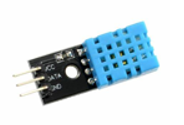
\includegraphics[width=0.3\textwidth]{figures/dht11}
    \caption{DHT11 温湿度传感器}\label{fig:4}
    \end{figure}

    \item {人体红外感应模块}:
    
    在对室内的部分设备进行控制的内容设计上,我们主要设计的是对led灯的开关控制功能,通过连接到ESP8266 WiFi局域网上,可以通过移动端手机app或者是PC端的web网页对led灯的开关进行远程控制。除了可以使用远程开关对led进行控制,我们还设计了“人过灯亮、人走灯灭”的自动开关灯,主要是通过传感器HC-SR501 人体红外感应模块(实物如下)采集红外感应数据,并让程序对获取的数据进行分析,实现自动的开关灯。
    \begin{figure}[htbp]
    \centering
    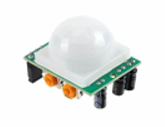
\includegraphics[width=0.3\textwidth]{figures/hongwai}
    \caption{HC-SR501 人体红外感应模块}\label{fig:5}
    \end{figure}

    \item {灰尘传感器}:
    
    室内环境状况检测的功能中,我们还设计了室内烟霾指数的测量与记录功能。主要使用的是传感器GP2Y1010AU0F 灰尘传感器(实物如下图),这个传感器可以检测室内空气中的灰尘与烟霾浓度,并将采集到的实时数据通过ESP8266传回app与web网页进行显示。与温度和湿度数据的采集和记录方式类似,除了获取当前的烟霾指数数据,我们同样设计了用于显示数据变化的折线图,在移动端app和web端上分别按照一定时间间隔绘制历史数据折线图,可以直观地反映烟霾指数变化情况。
    \begin{figure}[htbp]
    \centering
    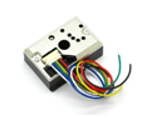
\includegraphics[width=0.3\textwidth]{figures/huichen}
    \caption{GP2Y1010AU0F 灰尘传感器}\label{fig:6}
    \end{figure}

    \item {火焰传感器+蜂鸣器}:
    
    最后一项功能是火灾报警装置。我们设计了结合蜂鸣器和火焰传感器(实物如下图)的火灾报警装置,火焰传感器获取室内烟雾和温度等数据,并判断是否室内起火,如果确定起火则将信号传递给蜂鸣器,触发蜂鸣器发出警报。

    \begin{figure}
        \centering
        \begin{minipage}{0.4\textwidth}
            \centering
            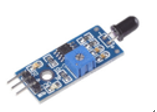
\includegraphics[width=0.5\textwidth]{figures/huoyan}
            \caption{火焰传感器}\label{fig:7}    
        \end{minipage}
        \begin{minipage}{0.4\textwidth}
            \centering
            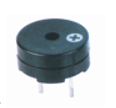
\includegraphics[width=0.4\textwidth]{figures/fengming}
            \caption{蜂鸣器}\label{fig:8}    
        \end{minipage}
    \end{figure}
\end{enumerate}